\section{Interfaces de usuario}

A continuación se muestran las interfaces desarrolladas en PyQt5. Se busca mantener una estructura intuitiva y modular que facilite la configuración, ejecución y visualización de los autómatas celulares.

\begin{itemize}
	\item \textbf{Pestaña de simulación}

	La pestaña de simulación permite configurar y controlar la evolución de los autómatas celulares, como se observa en la figura \ref{fig:ui_main}. Se divide en tres secciones: 
	
	\begin{figure}[H]
		\centering
		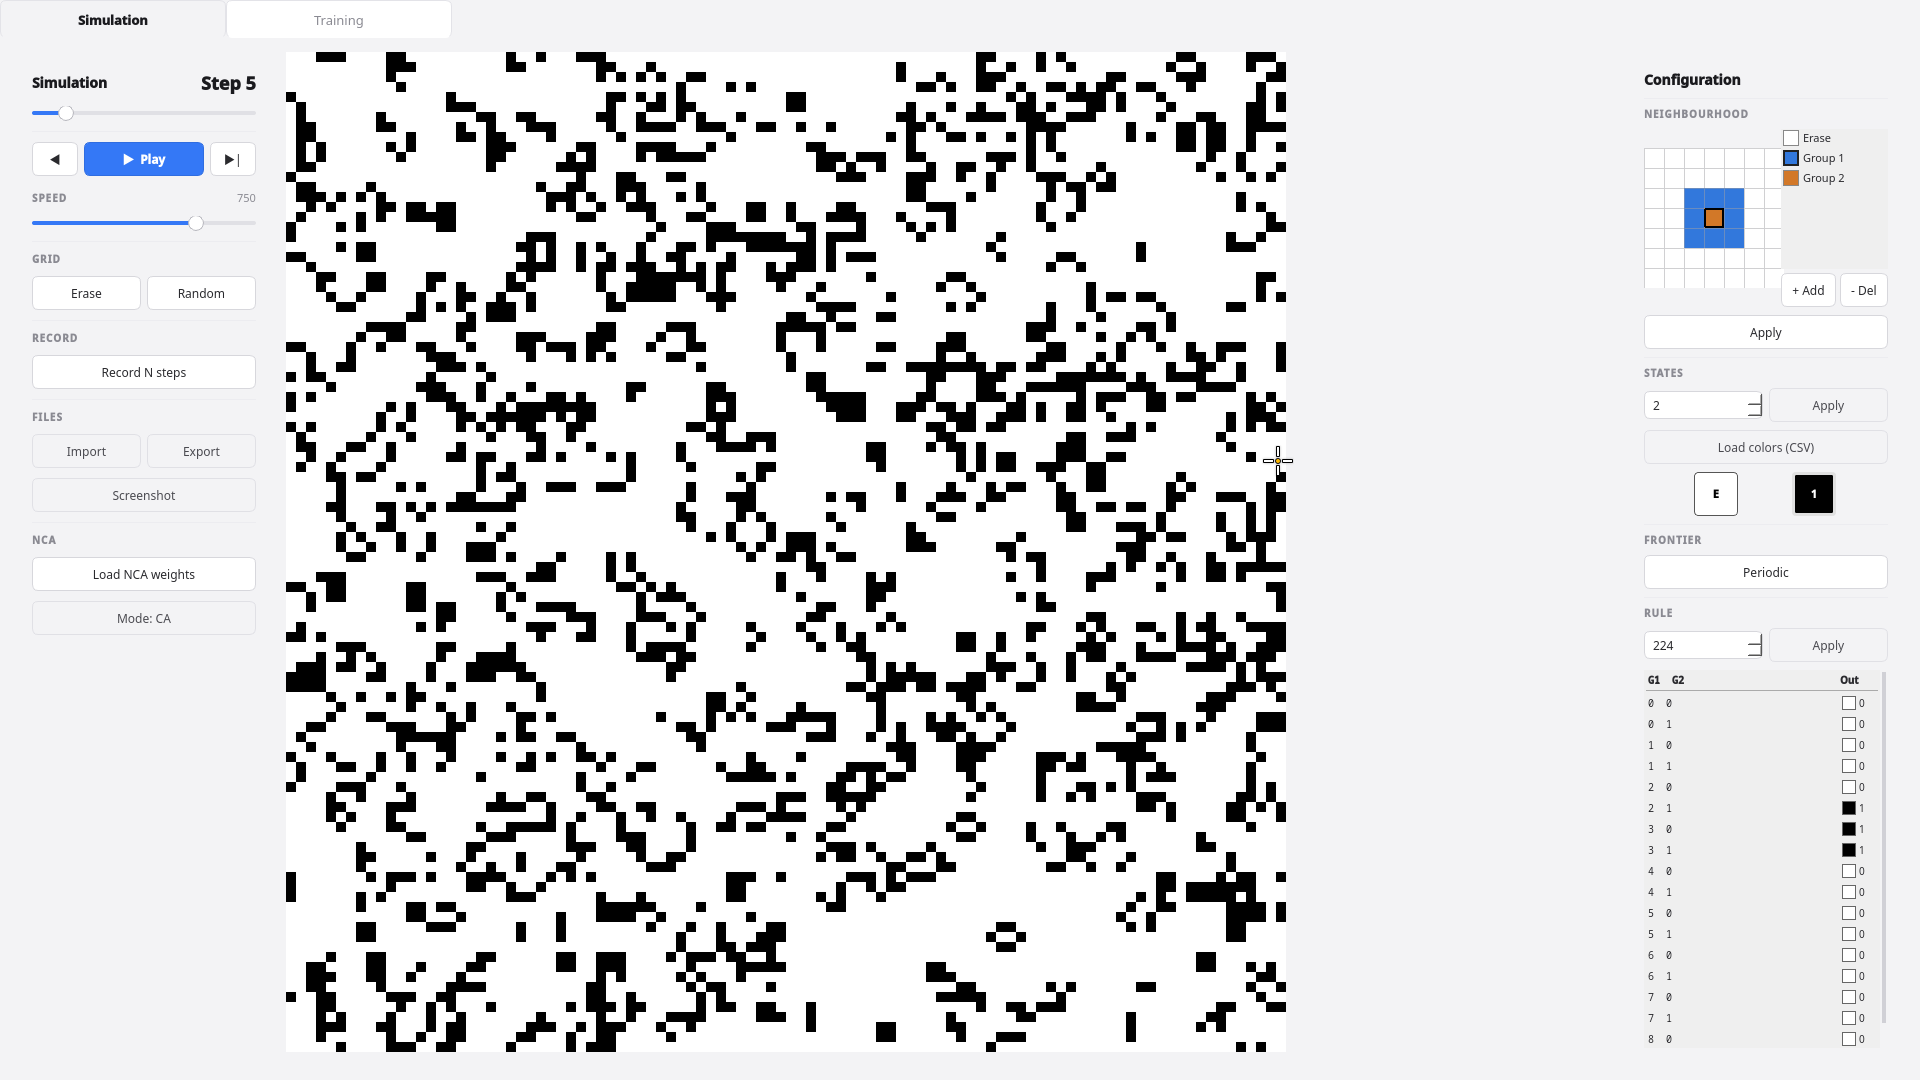
\includegraphics[width=0.9\linewidth]{img/disenoSoftware/ui_main.png}
		\caption{Interfaz de usuario. Pestaña de simulación.}
		\label{fig:ui_main}
	\end{figure}
	
	\begin{enumerate}
		\item Los controles de evolución, situados del lado izquierdo (ver figura \ref{fig:ui_main_simulator}), manipulan la evolución del autómata celular (iniciar, pausar, reiniciar, avanzar, retroceder o cambiar velocidad); además, permiten grabar un número de pasos, tomar capturas, importar y exportar evoluciones y cargar modelos del autómata celular neuronal.
		\item El área central es el espacio de evolución definido por una red regular cuadrada.
		\item La configuración del autómata celular, localizada del lado derecho (ver figura \ref{fig:ui_main_config}), define la vecindad, los estados, la condición de frontera y la regla de transición.
	\end{enumerate}
	
	\begin{figure}[H]
		\centering
		\begin{subfigure}{0.4\textwidth}
			\centering
			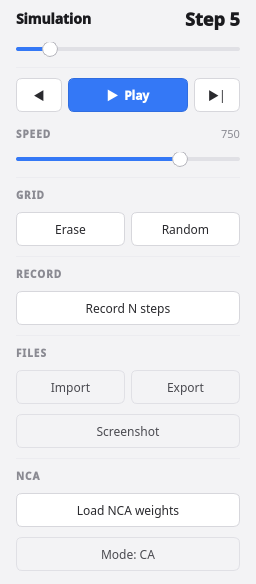
\includegraphics[width=0.8\linewidth]{img/disenoSoftware/ui_main_simulator.png}
			\caption{Controles de evolución.}
			\label{fig:ui_main_simulator}
		\end{subfigure}
		\begin{subfigure}{0.4 \textwidth}
			\centering
			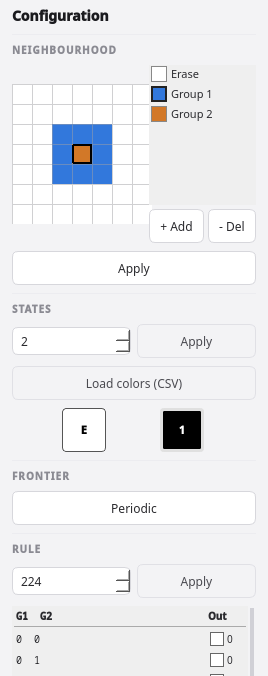
\includegraphics[width=0.8\linewidth]{img/disenoSoftware/ui_main_config.png}
			\caption{Controles de configuración.}
			\label{fig:ui_main_config}
		\end{subfigure}
	\end{figure}
	
	\item \textbf{Pestaña de entrenamiento}
	
	Esta pestaña permite al usuario entrenar el autómata celular neuronal dado un conjunto de datos, tal como se muestra en la figura \ref{fig:ui_training}. 
	
	\begin{figure}[H]
		\centering
		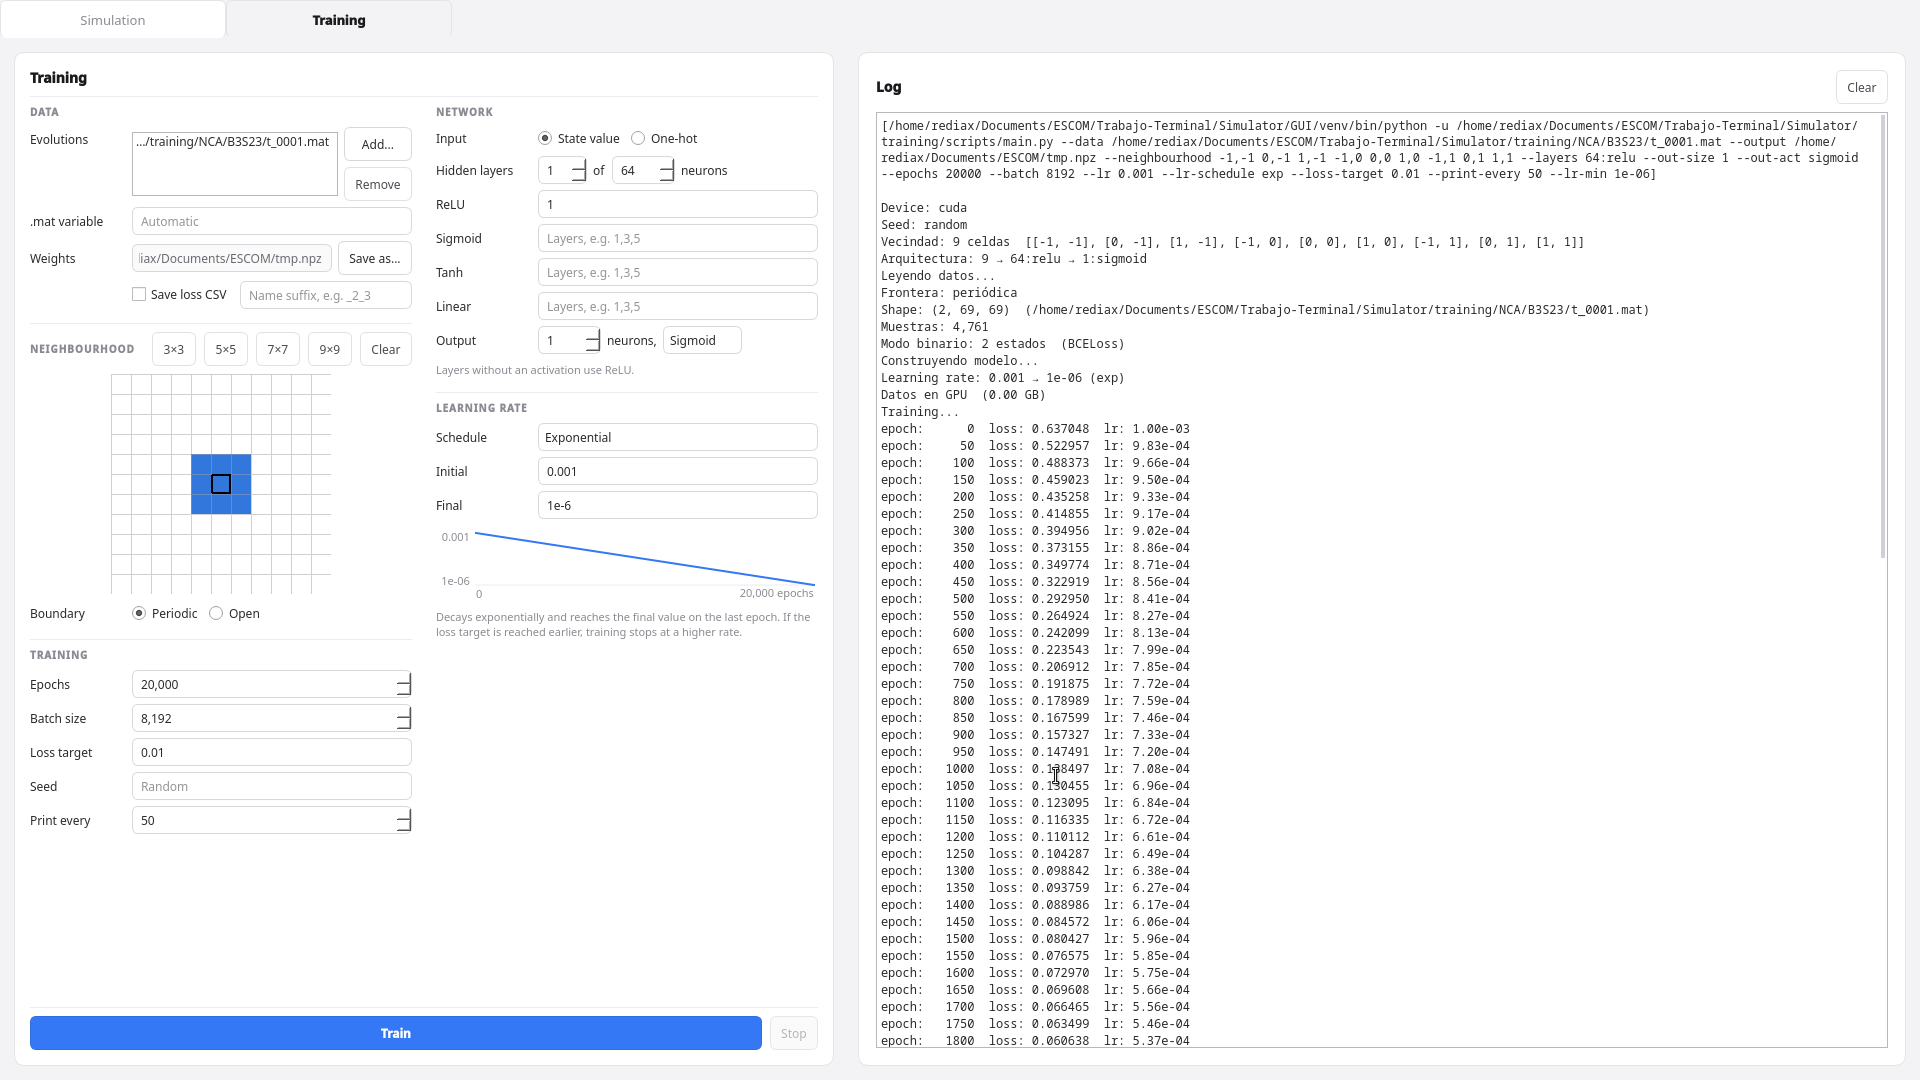
\includegraphics[width=0.9\linewidth]{img/disenoSoftware/ui_training.png}
		\caption{Interfaz de usuario. Pestaña de entrenamiento.}
		\label{fig:ui_training}
	\end{figure}
	
	La primera sección permite realizar la configuración, que incluye los datos de entrenamiento (una o varias evoluciones y el archivo de pesos), la vecindad y la condición de frontera, el número de capas ocultas y las funciones de activación de cada capa, así como la definición de hiperparámetros como el número de épocas, el tamaño del lote, la tasa de aprendizaje y su reducción, la pérdida objetivo y la semilla (ver figura \ref{fig:ui_training_config}). La segunda parte muestra únicamente los registros del entrenamiento. 
	
		\begin{figure}[H]
		\centering
		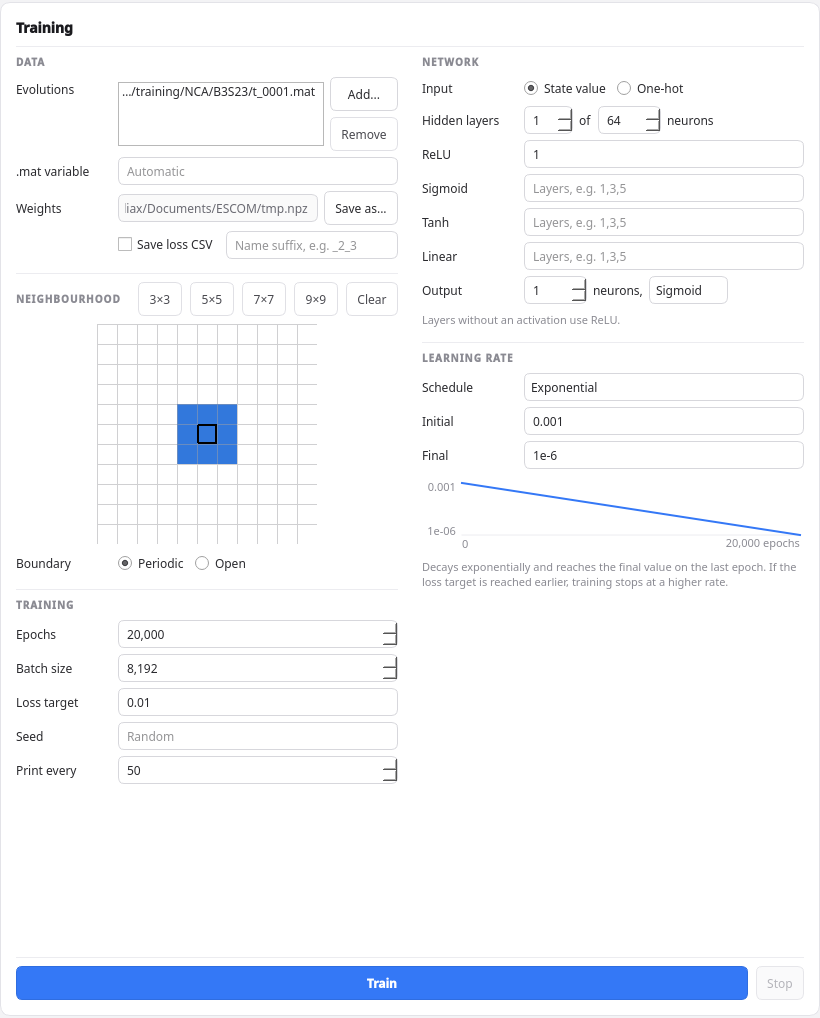
\includegraphics[width=0.8\linewidth]{img/disenoSoftware/ui_training_config.png}
		\caption{Controles de definición de entrenamiento.}
		\label{fig:ui_training_config}
	\end{figure}
\end{itemize}
